\documentclass{article}
\usepackage{tikz}
\usepackage{amsmath,amssymb}
\begin{document}

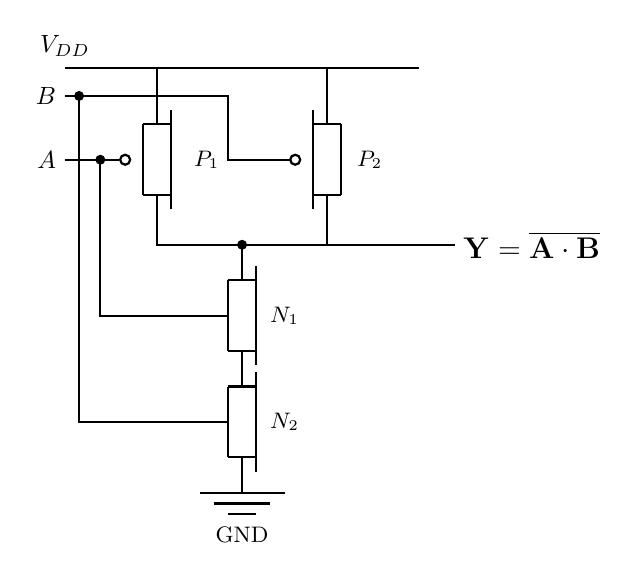
\begin{tikzpicture}[scale=0.9, transform shape]
  % Rails
  \draw[thick] (-2.5, 5.0) -- (2.5, 5.0);
  \node at (-2.5, 5.3) {$V_{DD}$};
  
  % PMOS P1 (Left)
  \draw[thick] (-1.2, 5.0) -- (-1.2, 4.2);
  \draw[thick] (-1.4, 4.2) -- (-1.0, 4.2);
  \draw[thick] (-1.4, 3.2) -- (-1.0, 3.2);
  \draw[thick] (-1.0, 4.4) -- (-1.0, 3.0);
  \draw[thick] (-1.4, 4.2) -- (-1.4, 3.2);
  \draw[thick] (-1.65, 3.7) circle (2pt);
  \draw[thick] (-2.5, 3.7) -- (-1.73, 3.7);
  \node[left] at (-2.5, 3.7) {$A$};
  \node at (-0.5, 3.7) {\small $P_1$};

  % PMOS P2 (Right)
  \draw[thick] (1.2, 5.0) -- (1.2, 4.2);
  \draw[thick] (1.0, 4.2) -- (1.4, 4.2);
  \draw[thick] (1.0, 3.2) -- (1.4, 3.2);
  \draw[thick] (1.0, 4.4) -- (1.0, 3.0);
  \draw[thick] (1.4, 4.2) -- (1.4, 3.2);
  \draw[thick] (0.75, 3.7) circle (2pt);
  \draw[thick] (0.67, 3.7) -- (-0.2, 3.7) -- (-0.2, 4.6) -- (-2.5, 4.6);
  \node[left] at (-2.5, 4.6) {$B$};
  \node at (1.8, 3.7) {\small $P_2$};

  % Common Drain Connection & Output
  \draw[thick] (-1.2, 3.2) -- (-1.2, 2.5) -- (1.2, 2.5) -- (1.2, 3.2);
  \draw[thick] (0, 2.5) -- (3.0, 2.5);
  \node[right] at (3.0, 2.5) {\large $\mathbf{Y = \overline{A \cdot B}}$};
  \fill (0, 2.5) circle (2pt);

  % NMOS N1 (Top Series)
  \draw[thick] (0, 2.5) -- (0, 2.0);
  \draw[thick] (-0.2, 2.0) -- (0.2, 2.0);
  \draw[thick] (-0.2, 1.0) -- (0.2, 1.0);
  \draw[thick] (0.2, 2.2) -- (0.2, 0.8);
  \draw[thick] (-0.2, 2.0) -- (-0.2, 1.0);
  \draw[thick] (-0.5, 1.5) -- (-0.2, 1.5);
  \draw[thick] (-0.5, 1.5) -- (-2.0, 1.5) -- (-2.0, 3.7);
  \fill (-2.0, 3.7) circle (2pt);
  \node at (0.6, 1.5) {\small $N_1$};

  % NMOS N2 (Bottom Series)
  \draw[thick] (0, 1.0) -- (0, 0.5);
  \draw[thick] (-0.2, 0.5) -- (0.2, 0.5);
  \draw[thick] (-0.2, -0.5) -- (0.2, -0.5);
  \draw[thick] (0.2, 0.7) -- (0.2, -0.7);
  \draw[thick] (-0.2, 0.5) -- (-0.2, -0.5);
  \draw[thick] (-0.5, 0.0) -- (-0.2, 0.0);
  \draw[thick] (-0.5, 0.0) -- (-2.3, 0.0) -- (-2.3, 4.6);
  \fill (-2.3, 4.6) circle (2pt);
  \node at (0.6, 0.0) {\small $N_2$};

  % Ground Rail
  \draw[thick] (0, -0.5) -- (0, -1.0);
  \draw[thick] (-0.6, -1.0) -- (0.6, -1.0);
  \draw[thick] (-0.4, -1.15) -- (0.4, -1.15);
  \draw[thick] (-0.2, -1.30) -- (0.2, -1.30);
  \node at (0, -1.6) {\small GND};
\end{tikzpicture}

\end{document}
